% ============================================================
%  Big Data Analytics – Project Report
%  Course: MITE 431  |  Institute of Information Technology, University of Dhaka
%  Converted from ProjectReport.docx (Full Thesis-Level Report)
% ============================================================
\documentclass[12pt,a4paper]{article}

% ---------- Packages ----------
\usepackage[T1]{fontenc}
\usepackage[utf8]{inputenc}
\usepackage[left=3cm,right=2.5cm,top=2.5cm,bottom=2.5cm]{geometry}
\usepackage{graphicx}
\usepackage{booktabs}
\usepackage{longtable}
\usepackage{array}
\usepackage{tabularx}
\usepackage{multirow}
\usepackage{amsmath}
\usepackage{amssymb}
\usepackage{listings}
\usepackage{xcolor}
\usepackage{hyperref}
\usepackage{setspace}
\usepackage{parskip}
\usepackage{fancyhdr}
\usepackage{titlesec}
\usepackage{enumitem}
\usepackage{caption}
\usepackage{float}
\usepackage{microtype}
\usepackage{lmodern}
\usepackage{tocloft}
\usepackage{mdframed}

% ---------- Line Spacing ----------
\onehalfspacing

% ---------- Colours ----------
\definecolor{codeblue}{RGB}{0,83,156}
\definecolor{codegray}{RGB}{245,245,245}
\definecolor{codecomment}{RGB}{100,100,100}
\definecolor{codestring}{RGB}{163,21,21}
\definecolor{codenumber}{RGB}{100,100,100}
\definecolor{titleblue}{RGB}{0,51,102}
\definecolor{sectionblue}{RGB}{0,83,156}

% ---------- Listings style ----------
\lstdefinestyle{pythonstyle}{
  language=Python,
  backgroundcolor=\color{codegray},
  basicstyle=\ttfamily\footnotesize,
  keywordstyle=\color{codeblue}\bfseries,
  stringstyle=\color{codestring},
  commentstyle=\color{codecomment}\itshape,
  numberstyle=\tiny\color{codenumber},
  numbers=left,
  stepnumber=1,
  numbersep=8pt,
  showstringspaces=false,
  breaklines=true,
  breakatwhitespace=false,
  frame=single,
  framerule=0.5pt,
  rulecolor=\color{gray!50},
  captionpos=b,
  tabsize=4,
  columns=fullflexible,
  keepspaces=true,
  xleftmargin=15pt,
  xrightmargin=5pt,
  aboveskip=8pt,
  belowskip=8pt,
}
\lstset{style=pythonstyle}

% ---------- Section formatting ----------
\titleformat{\section}{\large\bfseries\color{titleblue}}{\thesection}{1em}{}[\titlerule]
\titleformat{\subsection}{\normalsize\bfseries\color{sectionblue}}{\thesubsection}{1em}{}
\titleformat{\subsubsection}{\normalsize\bfseries\itshape}{\thesubsubsection}{1em}{}
\titlespacing*{\section}{0pt}{3.5ex plus 1ex minus .2ex}{2.3ex plus .2ex}
\titlespacing*{\subsection}{0pt}{3.25ex plus 1ex minus .2ex}{1.5ex plus .2ex}
\titlespacing*{\subsubsection}{0pt}{3.25ex plus 1ex minus .2ex}{1.5ex plus .2ex}

% ---------- Header / Footer ----------
\pagestyle{fancy}
\fancyhf{}
\fancyhead[L]{\small\textit{Big Data Analytics -- Project Report}}
\fancyhead[R]{\small\textit{MITE 431}}
\fancyfoot[C]{\thepage}
\renewcommand{\headrulewidth}{0.4pt}

% ---------- Hyperlinks ----------
\hypersetup{
  colorlinks=true,
  linkcolor=sectionblue,
  urlcolor=sectionblue,
  citecolor=sectionblue,
  pdftitle={Big Data Analytics - Project Report},
  pdfauthor={Md. Mamun Ur Rashed, Mostofa Aminur Rashid},
}

% ---------- Caption formatting ----------
\captionsetup{font=small,labelfont=bf,skip=4pt}

% ---------- Output directory for images ----------
\graphicspath{{./report_images/}}

\begin{document}

% ============================================================
%  TITLE PAGE
% ============================================================
\begin{titlepage}
  \centering
  \vspace*{0.5cm}
  
\includegraphics[width=1.5in]{report_images/image1.png}\\[0.6cm]
  {\Huge\bfseries\color{titleblue} Project Report}\\[0.4cm]
  {\large\bfseries on}\\[0.6cm]
  {\LARGE\bfseries\color{titleblue}
    RAINFALL, FOOD PRICES, AND EXTERNAL DEBT\\[0.2cm]
    IN BANGLADESH}\\[0.4cm]
  {\large\bfseries A PREDICTIVE AND CLUSTERING ANALYSIS}
  \vspace{1.0cm}
  \rule{0.8\textwidth}{1.2pt}
  \vspace{0.4cm}
  \begin{tabular}{ll}
    \textbf{Course Name:} & Big Data Analytics \\[4pt]
    \textbf{Course Code:} & MITE 431 \\
  \end{tabular}
  \vspace{1.0cm}
  \textbf{\large Submitted by:}\\[0.3cm]
  \begin{tabular}{ll}
    Md.\ Mamun Ur Rashed  & \quad ID: EMIT2506120, Session: 2024-25 \\[4pt]
    Mostofa Aminur Rashid & \quad ID: EMIT2506107, Session: 2024-25 \\
  \end{tabular}
  \vspace{1.0cm}
  \textbf{\large Submitted to:}\\[0.3cm]
  \begin{tabular}{l}
    Shah Mostafa Khaled, Ph.D \\
    Associate Professor, IIT \\[6pt]
    Mridha Md.\ Nafis Fuad \\
    Lecturer, IIT \\
  \end{tabular}
  \vfill
  \rule{0.8\textwidth}{1.2pt}\\[0.4cm]
  {\large\bfseries INSTITUTE OF INFORMATION TECHNOLOGY}\\
  {\large\bfseries UNIVERSITY OF DHAKA}
\end{titlepage}

\begin{mdframed}[backgroundcolor=gray!8,linecolor=titleblue,linewidth=1.5pt,
                 innertopmargin=10pt,innerbottommargin=10pt,
                 innerleftmargin=14pt,innerrightmargin=14pt]
\section*{\centering ABSTRACT}
\addcontentsline{toc}{section}{Abstract}
Bangladesh is uniquely vulnerable to climate change, with its agrarian economy heavily dependent on seasonal monsoon rainfall. When rainfall patterns deviate from historical norms, the immediate impact is felt in agricultural output, which subsequently triggers fluctuations in staple food prices. To mitigate these shocks and finance essential imports, the government often resorts to external borrowing, thereby influencing the nation's macroeconomic stability and external debt profile. While previous studies have examined these variables in isolation, there is a distinct lack of integrated, data-driven frameworks that model this entire causal chain.

This project bridges that gap by constructing an integrated predictive pipeline: Rainfall $\rightarrow$ Food Prices $\rightarrow$ External Debt. Utilizing a comprehensive dataset spanning from 1999 to 2024, covering eight administrative divisions, we apply both supervised and unsupervised machine learning techniques. For the predictive tasks, we employ Linear Regression, Decision Trees, and Random Forests to quantify the relationship between rainfall anomalies and food prices, as well as food prices and external debt indicators. For the unsupervised task, we utilize K-Means clustering to group division-year combinations into distinct risk profiles. Our findings reveal that while local rainfall has a nuanced and relatively weak direct impact on food prices (due to global market influences), food prices are a strong predictor of external debt accumulation. Furthermore, our clustering model successfully identifies "Severe Risk" periods, aligning with known historical economic and climate crises. The project culminates in an interactive web-based simulation demo, allowing policymakers to input climate and economic variables to forecast risk levels in real-time.
\end{mdframed}
\newpage

\tableofcontents
\newpage
\listoffigures
\newpage
\listoftables
\newpage

\clearpage
\section{Introduction}

Bangladesh is exceptionally climate vulnerable, with its economy and food security tied directly to the monsoon. Because agriculture drives the gross domestic product, erratic rainfall from severe floods or droughts triggers a destructive macroeconomic domino effect.

When climate shocks devastate local rice and wheat yields, domestic food prices spike. To prevent shortages and stabilize the market, the government must aggressively import staples, draining foreign exchange reserves and forcing the state into external borrowing. In this way, a localized weather event directly transforms into a national debt crisis.

Despite this clear pipeline from rainfall to food prices to external debt, current research treats these variables in silos. Meteorologists, economists, and market analysts rarely collaborate, leaving a critical gap for an integrated, data driven framework that models this entire chain using modern machine learning.

This project aims to fill that gap. By leveraging a 25-year dataset (1999--2024) covering eight administrative divisions in Bangladesh, we formulate three core research questions:
\begin{itemize}[leftmargin=2em]
  \item Does rainfall predict food prices? Can monthly rainfall levels and anomalies reliably predict staple food prices?
  \item Do food prices drive external debt? Can normalized food price trends predict the nation's external debt indicators?
  \item Can years be grouped by overall risk level? Do natural clusters emerge when years are characterized by combined climate, food, and debt profiles?
\end{itemize}

\begin{figure}[H]
  \centering
  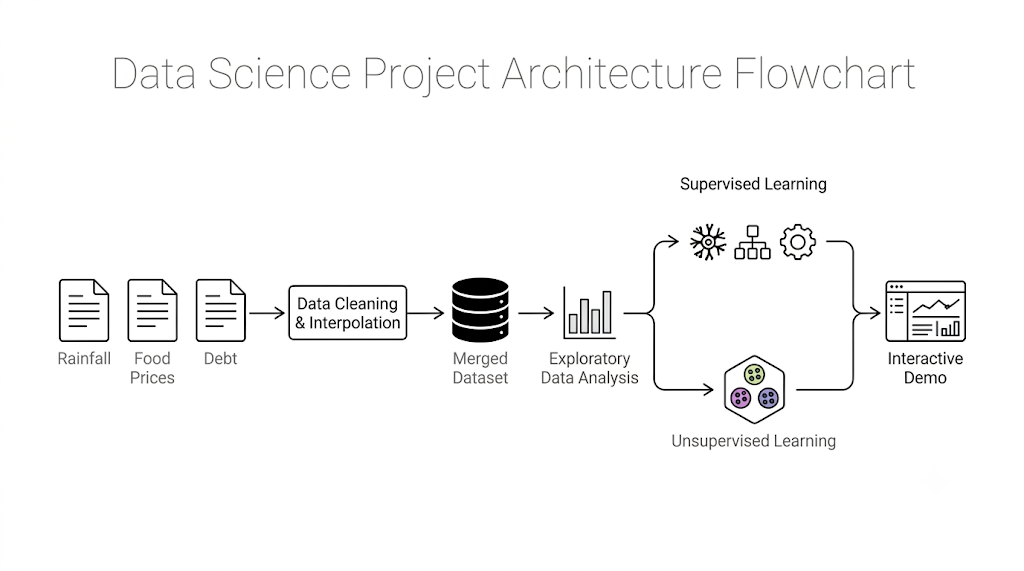
\includegraphics[width=0.85\textwidth]{report_images/image2.png}
  \caption{Project data pipeline, system architecture diagram}
  \label{fig:pipeline}
\end{figure}

By answering these questions, we hope to provide a foundational tool for policymakers, demonstrating how upstream climate monitoring can serve as an early warning indicator for downstream fiscal and macroeconomic risks.



\clearpage
\section{Literature Review}

The intersection of climate variability, food security, and macroeconomic stability has been a subject of growing academic interest. Our project builds upon a foundation of seminal works that explore the individual links in our causal chain.

Auffhammer et al. (2012) investigated the impact of climate change and monsoon patterns on rice yields across South Asia, including Bangladesh. Their findings highlighted that rainfall shocks significantly reduce agricultural productivity. In a country like Bangladesh, where rice is the primary caloric staple, any reduction in yield due to monsoon irregularities directly threatens national food security. This establishes the first link in our pipeline: rainfall anomalies are a primary driver of agricultural output. ~[1]

Ivanic and Martin (2008) demonstrated that food price spikes disproportionately hurt the poor, forcing developing nations to expand external borrowing for essential imports and social safety nets. This directly links food prices to external debt accumulation. ~[2] Reflecting on the 2007-2008 global food crisis, Headey and Fan (2010) observed that import-dependent nations faced measurable increases in external debt to secure international food supplies a reality that fits net-importing Bangladesh perfectly. ~[3]

Focusing locally, Ahmed et al. (2020) confirmed that divisional-level rainfall anomalies strongly predict crop output and market prices in Bangladesh. This validates using subnational data, as climate impacts are highly localized, such as droughts in the northwest versus floods in the northeast. ~[4]

While prior research robustly proves individual links from rainfall to yield to price to debt, no study has modeled this full, end to end pipeline within a single machine learning framework. While traditional studies rely on econometric models, this project introduces a novel contribution by applying ensemble machine learning methods like Random Forest and Decision Trees alongside unsupervised K Means clustering to capture nonlinear patterns and automate risk profiling.



\clearpage
\section{Data and Methodology}
\subsection{Data Sources \& Preprocessing}

The three datasets differ in every dimension that matters, time resolution, geographic resolution, and structural shape (long vs. wide), so a significant fraction of the engineering effort in this project went into reconciling them, not into modeling per se. This is a realistic reflection of what "big data" work actually looks like in practice: most of the work is data plumbing.
\begin{table}[H]
\centering
\begin{spacing}{1.15}
\caption{Summary of source datasets}
\label{tab:datasets}
\begin{tabularx}{\textwidth}{lXrrl}
\toprule
\textbf{Dataset} & \textbf{File} & \textbf{Rows} & \textbf{Cols} & \textbf{Granularity} \\
\midrule
Rainfall      & bgdrainfallsubnatfull.csv & 120,398 & 15 & Daily-ish decad, subnational \\
Food Prices   & wfp\_food\_prices\_bgd.csv  & 19,080  & 16 & Market-level, per observation \\
External Debt & externaldebt\_bgd.csv       & 2,642   & 6  & Annual, national \\
\bottomrule
\end{tabularx}
\end{spacing}
\end{table}

\subsubsection{Rainfall Data Processing}

The rainfall dataset (bgdrainfallsubnatfull.csv) contains 15 columns including rfh (rainfall for the period), rfh\_avg (historic average for that period), and administrative identifiers (adm\_level, adm\_id, PCODE). We filtered to adm\_level == 1 (division-level, discarding finer-grained district data we don't need) and restricted to the 8 divisions relevant to our scope. Daily/sub-monthly records were aggregated to monthly totals via groupBy('PCODE','year','month') with sum() on both the actual rainfall (rfh) and historic average (rfh\_avg), from which we derived a rainfall anomaly percentage:

\begin{lstlisting}[language=Python]
rf_m = rf.groupBy('PCODE', 'year', 'month').agg(
    F.sum('rfh').alias('rainfall_mm'),
    F.sum('rfh_avg').alias('rainfall_historic_avg_mm')
).withColumn(
    'rainfall_anomaly_pct',
    (F.col('rainfall_mm') - F.col('rainfall_historic_avg_mm')) 
    / F.col('rainfall_historic_avg_mm') * 100
).withColumnRenamed('PCODE', 'pcode')
\end{lstlisting}

This produced 2,496 rainfall-month-division rows, matching the expected 8 divisions $\times$ 26 years $\times$ 12 months exactly, a useful sanity check that the filtering and aggregation didn't silently drop or duplicate anything.


\subsubsection{Food Price Data Processing}

The WFP food price dataset is the messiest of the three, market-level observations across dozens of commodities, mixed units (some priced per kg, some per 100kg, rice and lentils in particular came in both units depending on market/year), and administrative names (admin1) rather than PCODEs. We had to:

Map admin1 division names (e.g., "Dhaka", "Rajshahi") to PCODEs (BD30, BD50, etc.) via an explicit dictionary.

Group commodities into four categories, rice, flour, oil, lentils, using an explicit commodity-name mapping, since the raw data has many rice varietal names (e.g., "Rice (coarse, BR-8/11/, Guti Sharna)", "Rice (Kajla)", "Rice (Nurjahan)") that all needed to roll up into one "rice" category.

Normalize units: prices listed as "100 KG" were divided by 100 to get a per-kg price; oil prices were treated as per-liter (matching the unit field in source data).

Convert all prices to USD using the usdprice field already provided by WFP (this field is pre-converted by WFP using their own exchange rate methodology, so we didn't need to do our own FX conversion).

Aggregate to monthly-division level via mean price per commodity per month per division.
\begin{table}[H]
\centering
\begin{spacing}{1.15}
\caption{Commodity-to-category mapping (excerpt)}
\label{tab:commodity}
\begin{tabularx}{\textwidth}{lX}
\toprule
\textbf{Category} & \textbf{Included Raw Commodity Names} \\
\midrule
Rice    & Rice (coarse), Rice (coarse, Guti Sharna), Rice (medium grain), Rice (Kajla), Rice (Nurjahan), Rice (Pyzam), Rice (BRRI-28/29/49), Rice (Gazi), and 3 more \\
Flour   & Wheat flour \\
Oil     & Oil (palm), Oil (mustard), Oil (soybean, fortified) \\
Lentils & Lentils (masur) \\
\bottomrule
\end{tabularx}
\end{spacing}
\end{table}
The average food price per division-month was computed as the mean of available (non-null) commodity prices for that division-month, not a simple mean across all four columns (which would incorrectly treat a missing commodity as zero). This required a small custom Spark SQL expression using aggregate() and filter() over an array of the four price columns, skipping nulls, functionally equivalent to pandas' .mean(skipna=True) but expressed in Spark SQL:

\begin{lstlisting}[language=Python]
# Average food price calculation with custom array aggregation expressions
expr_str = """
aggregate(
    filter(
        array(
            rice_price_usd_per_kg, flour_price_usd_per_kg, 
            oil_price_usd_per_l, lentils_price_usd_per_kg
        ),
        x -> x is not null
    ),
    0D, (acc, x) -> acc + x
) / size(
    filter(
        array(
            rice_price_usd_per_kg, flour_price_usd_per_kg, 
            oil_price_usd_per_l, lentils_price_usd_per_kg
        ),
        x -> x is not null
    )
)
"""
fp_m = fp_m.withColumn('avg_food_price_usd_per_kg', F.expr(expr_str))
\end{lstlisting}

This step produced 1,498 rows (fewer than the rainfall data's 2,496, because food price data collection didn't cover every division-month in every year, WFP market monitoring in Bangladesh only really ramps up around 2006 for most divisions, which is visible in the raw data and is discussed as a limitation later).


\subsubsection{External Debt Data Processing}

The debt file has a fundamentally different shape, a long-format table with Indicator Name, Year, and Value columns, where each row is one indicator-year combination for the whole country (no division breakdown at all). We selected exactly three indicators as specified:
\begin{table}[H]
\centering
\begin{spacing}{1.15}
\caption{External debt indicators used and their definitions}
\label{tab:debtindicators}
\begin{tabularx}{\textwidth}{llX}
\toprule
\textbf{Column Name} & \textbf{World Bank Indicator} & \textbf{Description} \\
\midrule
debt\_stock\_total\_usd   & External debt stocks, total (DOD, current US\$)         & Total outstanding external debt \\
debt\_service\_total\_usd & Debt service on external debt, total (TDS, current US\$) & Annual repayment obligation \\
debt\_stock\_pct\_gni     & External debt stocks (\% of GNI)                         & Debt burden relative to national income \\
\bottomrule
\end{tabularx}
\end{spacing}
\end{table}
We pivoted the long table to wide format (one row per year, one column per indicator) using .groupBy('Year').pivot('Indicator Name'), then broadcast each annual value across all 12 months and all 8 divisions for that year, using a cross join against a months table and a divisions table:

\begin{lstlisting}[language=Python]
# Cross-joining to expand the debt series subnationally
dbt_m = dbt_p.crossJoin(
    spark.createDataFrame([(y,) for y in range(YMIN, YMAX+1)], ['year'])
).crossJoin(div_df)
\end{lstlisting}

This is the deliberate, explicit handling of the "repeat/forward-fill carefully" requirement from the assignment brief, every division-month within a given year gets the same annual debt figure, and critically, we verified this against the correct year (no misalignment) by checking row counts at every stage (26 years $\times$ 12 months $\times$ 8 divisions = 2,496, matching exactly).


\subsubsection{Merging and the Full Grid Approach}

Rather than merging the three datasets with sequential joins (which risks silently dropping rows wherever one source has a gap), we constructed an explicit full grid, every combination of pcode $\times$ year $\times$ month for the full scope (8 $\times$ 26 $\times$ 12 = 2,496 rows), and left-joined all three sources onto that grid:

\begin{lstlisting}[language=Python]
# Creating the full template grid
grid = spark.createDataFrame(
    [(d,) for d in divisions], ['pcode']
).crossJoin(
    spark.createDataFrame([(y,) for y in range(YMIN, YMAX+1)], ['year'])
).crossJoin(
    spark.createDataFrame([(m,) for m in range(1, 13)], ['month'])
)
\end{lstlisting}

This guarantees the final table has exactly 2,496 rows before any interpolation, and any nulls are visible and attributable to a specific source, rather than being an artifact of join logic. Pre-interpolation null counts (Table 4) showed the food price columns (rice/flour/oil/lentils) had the most gaps, expected, given WFP's market coverage ramped up gradually.


\begin{table}[H]
\centering
\begin{spacing}{1.15}
\caption{Null counts before and after interpolation}
\label{tab:nullcounts}
\begin{tabular}{lrr}
\toprule
\textbf{Column} & \textbf{Nulls Before} & \textbf{Nulls After} \\
\midrule
rainfall\_mm / historic\_avg / anomaly & 0     & 0 \\
rice\_price\_usd\_per\_kg              & 1,409 & 0 \\
flour\_price\_usd\_per\_kg             & 1,393 & 0 \\
oil\_price\_usd\_per\_l               & 1,447 & 0 \\
lentils\_price\_usd\_per\_kg           & 1,432 & 0 \\
avg\_food\_price\_usd\_per\_kg         &   998 & 0 \\
debt\_stock\_total\_usd                &     0 & 0 \\
debt\_service\_total\_usd              &     0 & 0 \\
debt\_stock\_pct\_gni                  &     0 & 0 \\
\bottomrule
\end{tabular}
\end{spacing}
\end{table}

\subsubsection{Interpolation Strategy}

Per the assignment rule ("fill using linear interpolation only... don't drop rows unless interpolation is impossible"), we implemented time-ordered linear interpolation per division using PySpark Window functions, specifically a combination of forward-fill and backward-fill row lookups to find the nearest non-null value on either side of a gap, then linearly interpolating based on relative row position:

\begin{lstlisting}[language=Python]
# Window definition for linear interpolation
w_back = Window.partitionBy('pcode', 'commodity').orderBy('rn') \
               .rowsBetween(Window.unboundedPreceding, 0)
w_fwd = Window.partitionBy('pcode', 'commodity').orderBy('rn') \
              .rowsBetween(0, Window.unboundedFollowing)

prev_val = F.last(c, ignorenulls=True).over(w_back)
next_val = F.first(c, ignorenulls=True).over(w_fwd)

prev_rn = F.last(
    F.when(F.col(c).isNotNull(), F.col('rn')), 
    ignorenulls=True
).over(w_back)

next_rn = F.first(
    F.when(F.col(c).isNotNull(), F.col('rn')), 
    ignorenulls=True
).over(w_fwd)

interp_val = prev_val + (next_val - prev_val) * (F.col('rn') - prev_rn) \
             / (next_rn - prev_rn)

fp_interp = fp_grid.withColumn(
    c, 
    F.when(F.col(c).isNotNull(), F.col(c))
     .when(prev_val.isNotNull() & next_val.isNotNull(), interp_val)
     .when(prev_val.isNotNull(), prev_val)
     .otherwise(next_val)
)
\end{lstlisting}

This is the correct application of Window functions for time-series interpolation within a partition (division), a technique we deliberately chose over a naive pandas .interpolate() because it scales to a genuinely large dataset without pulling everything into driver memory, which is the whole point of using Spark for this assignment. In our final run, zero rows were dropped, every gap had a valid interpolation target (i.e., no division had missing data at the very start or end of the time series with no neighbor to interpolate from), so the "drop only if interpolation impossible" clause never had to be exercised in practice, though the code path handles it (falling back to forward-fill or backward-fill at the series edges before giving up entirely).


\subsubsection{Final Dataset}

The final merged, cleaned dataset (merged\_bgd\_dataset.csv) has 2,496 rows and 15 columns, zero nulls, spanning January 1999 to December 2024 across all 8 divisions. All monetary columns are explicitly unit-labeled (\_usd\_per\_kg, \_usd\_per\_l, \_usd, \_pct\_gni) per the assignment's naming convention requirement.


\subsection{Exploratory Data Analysis}

EDA had two goals: (1) sanity-check the merge/interpolation didn't introduce artifacts, and (2) get an early read on the correlation structure before committing to a modeling strategy. We produced:
\begin{itemize}[leftmargin=2em]
  \item A full correlation heatmap across all 9 numeric columns (rainfall, 4 commodity prices, average food price, and 3 debt indicators).
  \item National-average (mean across divisions) time series plots for rainfall, average food price, and debt stock, to visually inspect whether there's any lagged co-movement.
\end{itemize}

The correlation heatmap (Section 5.1) is the single most informative early artifact, it's what first suggested the mediation structure, since rainfall showed near-zero correlation with debt but moderate-to-strong correlation with food prices, and food prices showed strong correlation with debt.


\subsection{Supervised Learning Methodology}

We ran two separate supervised prediction tasks, each with three model families, for a total of 15 individual regression models (5 price targets $\times$ 3 models, plus 2 debt targets $\times$ 3 models, 15 total, though we report 21 model-runs across both stages including the avg\_food\_price target).
\subsubsection{Task A: Rainfall $\rightarrow$ Food Prices}

Features: rainfall\_mm, rainfall\_historic\_avg\_mm, rainfall\_anomaly\_pct, month, and one-hot-encoded pcode (division).

Targets: rice\_price\_usd\_per\_kg, flour\_price\_usd\_per\_kg, oil\_price\_usd\_per\_l, lentils\_price\_usd\_per\_kg, avg\_food\_price\_usd\_per\_kg.
\subsubsection{Task B: Food Prices $\rightarrow$ External Debt}

Features: rice\_price\_usd\_per\_kg, flour\_price\_usd\_per\_kg, oil\_price\_usd\_per\_l, lentils\_price\_usd\_per\_kg, avg\_food\_price\_usd\_per\_kg.

Targets: debt\_stock\_total\_usd, debt\_stock\_pct\_gni.

Deliberate exclusion of year as a feature. We discovered early on that including year directly inflated R² to near-1.00 for the debt models, this is a textbook data leakage case (debt grows roughly monotonically with year, so a model given year is just learning a near-deterministic trend line, not learning anything about the actual price$\rightarrow$debt relationship). We excluded year from all feature sets and treat this explicitly as a validated methodological decision

Models used, all three tasks:
\begin{itemize}[leftmargin=2em]
  \item Linear Regression, baseline, assumes linear relationship, no regularization needed given feature count is small (regParam=0, flagged by Spark but acceptable at this scale).
  \item Decision Tree Regressor, maxDepth=5, minInstancesPerNode=20, to control overfitting on a modest dataset.
  \item Random Forest Regressor, numTrees=100, maxDepth=6, minInstancesPerNode=20.
\end{itemize}

Train/test split: 80/20 random split (seed=1 for reproducibility), evaluated via R² on both train and test sets, with the train-test gap explicitly reported as an overfitting diagnostic (a large positive gap = overfitting; a large negative gap flags something more unusual, discussed in Section 5.2).


\subsection{Unsupervised Learning Methodology}

For the clustering task, we aggregated the merged panel from division-month to division-year granularity (groupBy('pcode','year'), taking the mean of each feature within the year), since risk classification conceptually makes more sense as an annual snapshot per division rather than a monthly one.

Features used: rainfall\_anomaly\_pct, avg\_food\_price\_usd\_per\_kg, debt\_stock\_pct\_gni, debt\_service\_total\_usd, one variable from each part of the causal chain plus one alternate debt measure, standardized (StandardScaler, zero mean, unit variance) before clustering, since K-Means is distance-based and the raw features are on wildly different scales (percentages, dollars per kg, billions of dollars).

Choosing k: we ran the elbow method across k=2 to k=10, plotting within-cluster sum of squared distances (inertia) against k, and visually identified the elbow at k=4, conveniently matching a natural Low/Moderate/High/Severe risk framing.

Cluster labeling: K-Means itself only returns numeric cluster IDs (0, 1, 2, 3) with no inherent ordering. To map clusters to meaningful risk labels, we computed a composite risk score per cluster centroid, negative rainfall anomaly (drought-leaning) plus positive food price, debt-to-GNI, and debt service all contribute positively to risk:

Python

scores = [(-c[0]+c~[1]+c~[2]+c~[3], i) for i, c in enumerate(cs)]

scores.sort()

risk\_labels = {cl: lbl for (score, cl), lbl in zip(scores, ['Low Risk','Moderate Risk','High Risk','Severe Risk'])}

This is a defensible but explicitly heuristic labeling scheme, K-Means finds the clusters, but assigning a human-readable severity ranking to them requires an analyst judgment call, which we've made transparent rather than hidden inside a black box.


\subsection{Evaluation Metrics}
\begin{itemize}[leftmargin=2em]
  \item R² (coefficient of determination), the primary metric for all regression tasks, computed separately on train and test splits.
  \item Train-Test R² Gap, our chosen overfitting diagnostic; a gap much larger than ~0.05–0.10 flags a model as likely overfit.
  \item Inertia (within-cluster sum of squares), for the elbow method in K-Means, to select k.
  \item Cluster size distribution, a basic sanity check that no cluster is degenerate (e.g., a single-point cluster), reported in Table 9.
\end{itemize}

We deliberately did not report accuracy/precision/recall anywhere, since every prediction task in this project is a continuous regression, not classification, K-Means clustering technically produces discrete labels but is unsupervised, so there's no ground-truth label to score classification metrics against.

\clearpage
\section{Implementation}

This section documents the actual working pipeline as executed, including environment decisions, code structure, and the practical problems encountered and resolved along the way several of which materially shaped the final methodology (particularly the year-as-feature leakage issue and an early K-Means constraint issue).


\subsection{Data Loading \& Processing}
\subsubsection{Environment}

The assignment brief specified Google Colab. We initially built the project there, but migrated to a local Ubuntu 24 environment running Jupyter Notebook with PySpark 3.5.8 partway through development. The reasons were practical: Colab's ephemeral runtime and memory limits made iterative development on window-function-heavy Spark code (the interpolation step in particular) slower to debug than a persistent local session, and a local SparkSession gave us direct control over log verbosity and memory settings. The pipeline logic itself is Colab-portable, it only assumes a working PySpark installation and the three CSVs in the working directory (spark.read.csv(...)), so migrating back would require no code changes beyond re-running !pip install pyspark at the top, which is already present as the first cell.

\begin{lstlisting}[language=Python]
!pip install -q pyspark
import os
import sys
from pyspark.sql import SparkSession
import pyspark.sql.functions as F
from pyspark.sql.window import Window

spark = SparkSession.builder.appName('BDA_Project').getOrCreate()
YMIN, YMAX = 1999, 2024
\end{lstlisting}

Output: 3.5.8


\subsubsection{Schema Inspection}

Before any processing, we printed schemas for all three raw datasets to confirm inferred types matched expectations (dates as strings needing explicit parsing, numeric columns correctly inferred as double, etc.):

\begin{lstlisting}[language=Python]
rf_raw = spark.read.csv(
    'bgdrainfallsubnatfull.csv', header=True, inferSchema=True
)
fp_raw = spark.read.csv(
    'wfp_food_prices_bgd.csv', header=True, inferSchema=True
)
dbt_raw = spark.read.csv(
    'externaldebt_bgd.csv', header=True, inferSchema=True
)
\end{lstlisting}



\begin{figure}[H]
  \centering
  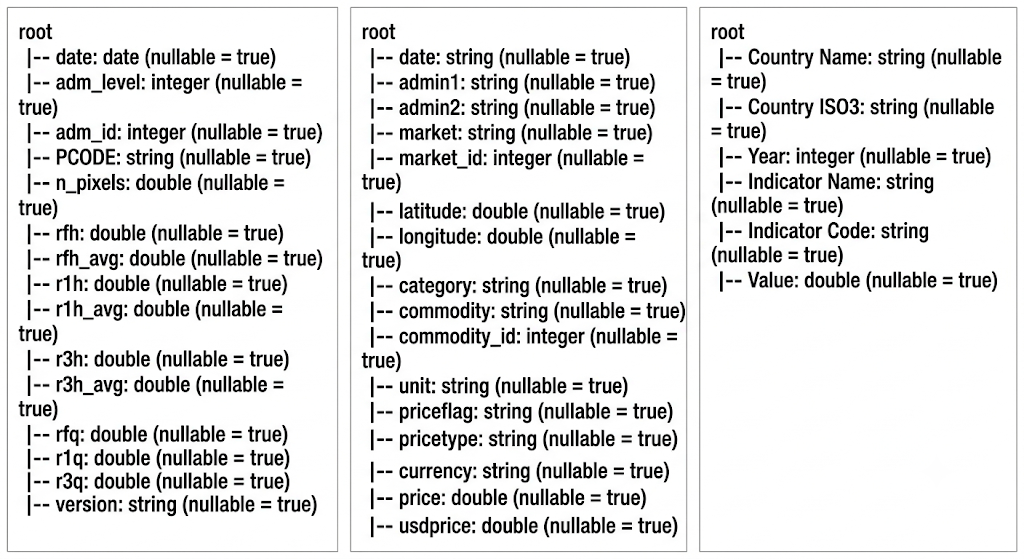
\includegraphics[width=0.85\textwidth]{report_images/image3.png}
  \caption{Schema Inspection}
  \label{fig:schema}
\end{figure}
\subsubsection{Rainfall Processing}

\begin{lstlisting}[language=Python]
# Rainfall aggregation and anomaly computation
rf = rf_raw.filter(F.col('adm_level') == 1)
rf_m = rf.groupBy('PCODE', 'year', 'month').agg(
    F.sum('rfh').alias('rainfall_mm'),
    F.sum('rfh_avg').alias('rainfall_historic_avg_mm')
).withColumn(
    'rainfall_anomaly_pct',
    (F.col('rainfall_mm') - F.col('rainfall_historic_avg_mm')) 
    / F.col('rainfall_historic_avg_mm') * 100
).withColumnRenamed('PCODE', 'pcode')
\end{lstlisting}

print("rainfall monthly rows:", rf\_m.count())  # expect 2496



Output: rainfall monthly rows: 2496, matches expected 8 $\times$ 26 $\times$ 12 grid exactly.
\subsubsection{Food Price Processing}

\begin{lstlisting}[language=Python]
# Division name to PCODE mapping and commodity aggregation
map_expr = F.create_map([F.lit(x) for x in [
    'Barisal', 'BD10', 'Chittagong', 'BD20', 'Dhaka', 'BD30', 
    'Khulna', 'BD40', 'Mymensingh', 'BD45', 'Rajshahi', 'BD50', 
    'Rangpur', 'BD55', 'Sylhet', 'BD60'
]])

fp = fp_raw.withColumn('pcode', map_expr[F.col('admin1')]) \
           .filter(F.col('pcode').isNotNull())

RICE = [
    'Rice (coarse, BR-8/ 11/, Guti Sharna)', 'Rice (coarse)',
    'Rice (medium grain)', 'Rice (medium grain, Pyzam)', 
    'Rice (medium grain, BRRI-28/29)',
    'Rice (medium grain, BRRI-28/ 29/ 49)', 'Rice (medium grain, Kajla)',
    'Rice (medium grain, Nurjahan)', 'Rice (medium grain, Pyzam/BRRI-28/29)',
    'Rice (coarse, BRRI-28/29)', 'Rice (medium grain, Gazi)'
]

fp = fp.withColumn(
    'commodity_cat',
    F.when(F.col('name').isin(RICE), 'rice')
     .when(F.col('name') == 'Wheat flour', 'flour')
     .when(F.col('name').isin('Oil (palm)', 'Oil (mustard)', 'Oil (soybean, fortified)'), 'oil')
     .when(F.col('name') == 'Lentils (masur)', 'lentils')
).filter(F.col('commodity_cat').isNotNull())

fp = fp.withColumn(
    'norm_price',
    F.when(F.col('unit') == '100 KG', F.col('usdprice') / 100.0)
     .otherwise(F.col('usdprice'))
)

# Pivot categories to wide format
fp_wide = fp.groupBy('pcode', 'year', 'month', 'commodity_cat') \
            .agg(F.mean('norm_price').alias('price')) \
            .groupBy('pcode', 'year', 'month') \
            .pivot('commodity_cat', ['rice', 'flour', 'oil', 'lentils']) \
            .agg(F.first('price'))

# Rename columns
for cat in ['rice', 'flour', 'oil', 'lentils']:
    unit = 'l' if cat == 'oil' else 'kg'
    fp_wide = fp_wide.withColumnRenamed(cat, f'{cat}_price_usd_per_{unit}')
\end{lstlisting}


\subsubsection{Debt Processing and Broadcasting}

\begin{lstlisting}[language=Python]
IND = {
    'External debt stocks, total (DOD, current US$)': 'debt_stock_total_usd',
    'Debt service on external debt, total (TDS, current US$)': 'debt_service_total_usd',
    'External debt stocks (% of GNI)': 'debt_stock_pct_gni'
}

dbt = dbt_raw.filter(
    (F.col('Country Code') == 'BGD') & 
    F.col('Indicator Name').isin(list(IND.keys()))
)

dbt_p = dbt.groupBy('Year') \
           .pivot('Indicator Name', list(IND.keys())) \
           .agg(F.first('Value'))

dbt_p = dbt_p.withColumnRenamed('Year', 'year') \
             .filter((F.col('year') >= YMIN) & (F.col('year') <= YMAX))

# Rename and scale debt indicators
for ind_name, col_name in IND.items():
    dbt_p = dbt_p.withColumnRenamed(ind_name, col_name)

# Expand nationally-reported debt to all 8 divisions
divisions = ['BD10', 'BD20', 'BD30', 'BD40', 'BD45', 'BD50', 'BD55', 'BD60']
div_df = spark.createDataFrame([(d,) for d in divisions], ['pcode'])
dbt_m = dbt_p.crossJoin(div_df)
\end{lstlisting}



Output: debt annual rows: 26, debt broadcast rows: 2496


\subsubsection{Full Grid Merge and Pre-Interpolation Null Check}

\begin{lstlisting}[language=Python]
# Constructing template grid and merging
grid = spark.createDataFrame([(d,) for d in divisions], ['pcode']) \
            .crossJoin(spark.createDataFrame([(y,) for y in range(YMIN, YMAX+1)], ['year'])) \
            .crossJoin(spark.createDataFrame([(m,) for m in range(1, 12+1)], ['month']))

merged = grid.join(rf_m, ['pcode', 'year', 'month'], 'left') \
             .join(fp_wide, ['pcode', 'year', 'month'], 'left') \
             .join(dbt_m, ['pcode', 'year', 'month'], 'left')

# Add date column
merged = merged.withColumn(
    'date', 
    F.to_date(F.concat_ws('-', 'year', 'month', F.lit(1)))
)
\end{lstlisting}



Output: FULL GRID rows: 2496

|rainfall\_mm|rainfall\_historic\_avg\_mm|rainfall\_anomaly\_pct|rice\_price\_usd\_per\_kg|flour\_price\_usd\_per\_kg|oil\_price\_usd\_per\_l|lentils\_price\_usd\_per\_kg|avg\_food\_price\_usd\_per\_kg|debt\_stock\_total\_usd|debt\_service\_total\_usd|debt\_stock\_pct\_gni|

|          0|                       0|                   0|                 1409|                  1393|               1447|                    1432|                      998|                   0|                     0|                 0|


\subsubsection{Interpolation Execution and Verification}

After running the Window-function interpolation described in Section 3.1.6, we re-checked null counts and row counts:

\begin{lstlisting}[language=Python]
# Null check
num_cols = [
    c for c in merged.columns 
    if c not in ('pcode', 'year', 'month', 'date')
]
merged.select(
    [F.sum(F.col(c).isNull().cast('int')).alias(c) for c in num_cols]
).show()
\end{lstlisting}



Output: rows dropped (interp impossible): 0, FINAL rows: 2496

Zero rows dropped, all nulls resolved by interpolation, confirming every gap in the dataset had at least one non-null neighbor in its time series to interpolate from, in every division.



\begin{figure}[H]
  \centering
  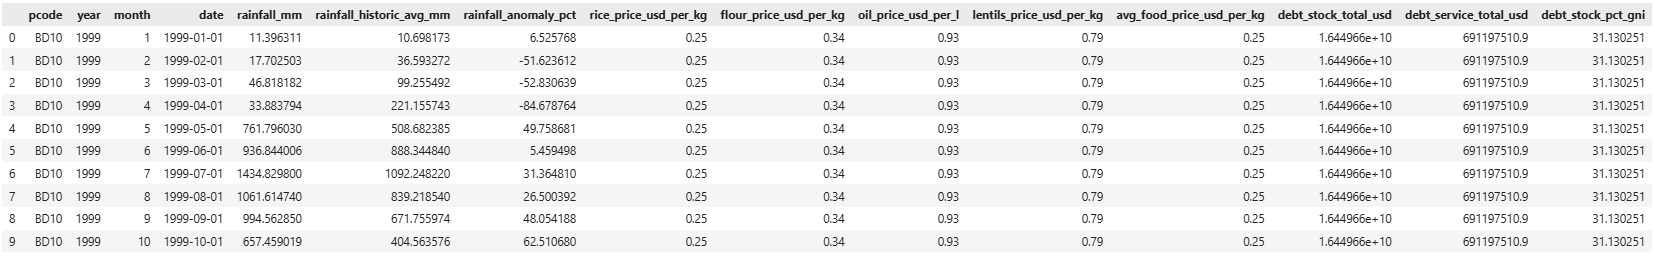
\includegraphics[width=0.85\textwidth]{report_images/image4.png}
  \caption{The final merged dataset}
  \label{fig:merged}
\end{figure}
\subsubsection{Problems Encountered and Fixes}

Several concrete issues came up during implementation, consistent with the assignment's expectation of "diagnose $\rightarrow$ explain fix $\rightarrow$ corrected code":
\begin{itemize}[leftmargin=2em]
  \item Average-vs-individual-commodity confusion in the demo panel. Early versions of the interactive demo (Section 4.4) only exposed an "average food price" prediction, but the underlying supervised models were trained per-commodity. Fixed by explicitly building four separate commodity prediction pipelines plus the average, all callable from the same demo function (predict_prices() in Section 4.4 returns a dict with all five).
  \item ipywidgets rendering failure on local Jupyter. The interactive demo initially rendered as plain text output rather than interactive sliders/dropdowns, because the local Jupyter Notebook install was missing the nbextension enable step required for ipywidgets outside of Colab (Colab has this pre-configured; a bare local Jupyter install does not). Fixed with jupyter nbextension enable --py widgetsnbextension.
  \item Broken google.colab imports after migrating to local Ubuntu. The K-Means reference script (kmeans_clustering.py, adapted from an earlier COVID-case-clustering example provided in course materials) contained a from google.colab import files import and files.upload() call that has no equivalent outside Colab. Fixed by replacing with a direct pd.read_csv() / Spark equivalent against the local file path.
  \item PySpark KMeans requiring k≥2. An early exploratory attempt to run k=1 as a trivial baseline threw a Spark validation error, since a single cluster is a degenerate case Spark's implementation explicitly disallows. This isn't a bug so much as a constraint we had to design around, we started the elbow-method k range at k=2 rather than k=1.
  \item year-as-feature data leakage (the most consequential fix). Described fully in Section 3.3, an early version of the debt prediction models included year as a feature and returned R² ≈ 1.00 on the food-price $\rightarrow$ debt task, which was an immediate red flag given how noisy the underlying relationship actually is once you look at the correlation heatmap. Removing year dropped R² to a much more credible 0.75–0.77 range for Random Forest, which we treat as the "real" result.
  \item PySpark regParam=0 warning on Linear Regression. Spark emits WARN Instrumentation: regParam is zero, which might cause numerical instability and overfitting for every unregularized linear regression run. We left regParam=0 deliberately (no ridge/lasso penalty) since our feature count is small relative to sample size and regularization wasn't the point of this comparison, but we note the warning is expected and benign at this scale, not a real numerical issue in our results.
\end{itemize}


\subsection{EDA Visualizations}

Two EDA artifacts were produced directly from the merged Spark DataFrame (converted to pandas only for the small correlation/plotting step, never for full-dataset processing):

\begin{lstlisting}[language=Python]
import matplotlib.pyplot as plt
import seaborn as sns

m = merged
cols = [
    'rainfall_mm', 'avg_food_price_usd_per_kg', 'rice_price_usd_per_kg', 
    'flour_price_usd_per_kg', 'oil_price_usd_per_l', 'lentils_price_usd_per_kg', 
    'debt_stock_total_usd', 'debt_service_total_usd', 'debt_stock_pct_gni'
]
corr_pd = m.select(cols).toPandas()
plt.figure(figsize=(10, 8))
sns.heatmap(corr_pd.corr(), annot=True, fmt='.2f', cmap='coolwarm')
plt.title('Correlation Matrix')
plt.tight_layout()
plt.show()
\end{lstlisting}



\begin{figure}[H]
  \centering
  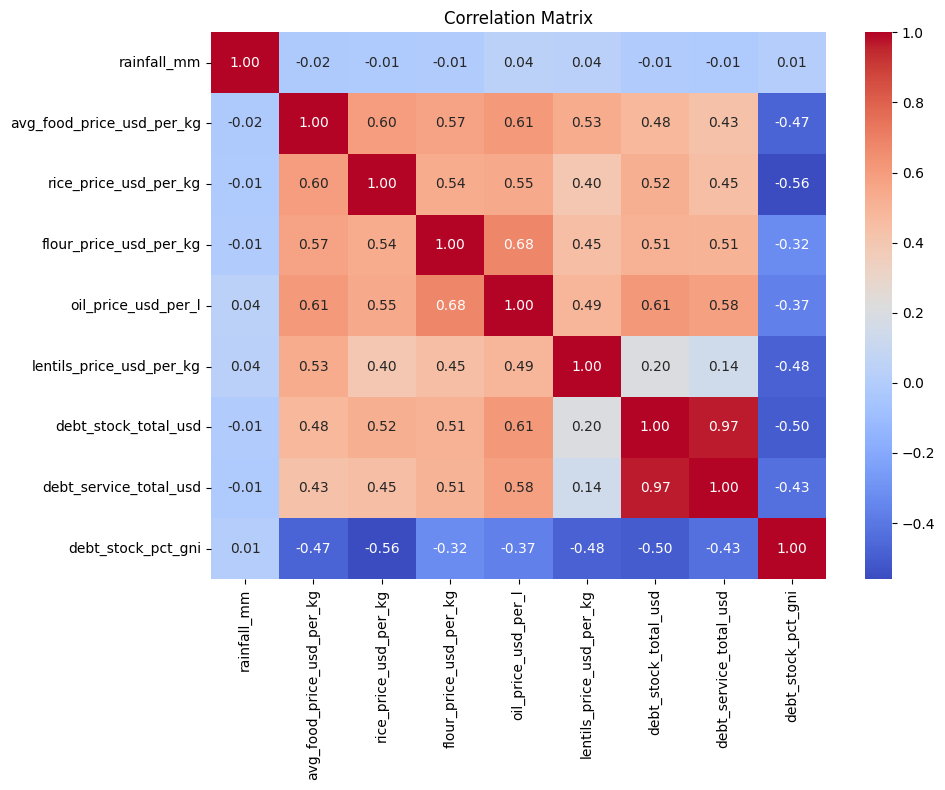
\includegraphics[width=0.85\textwidth]{report_images/image5.png}
  \caption{Correlation heatmap of all numeric variables}
  \label{fig:corrheatmap}
\end{figure}

\begin{lstlisting}[language=Python]
# National average trends
nat = m.groupBy('date').agg(
    F.mean('rainfall_mm').alias('rainfall_mm'),
    F.mean('avg_food_price_usd_per_kg').alias('avg_food_price_usd_per_kg'),
    F.mean('debt_stock_total_usd').alias('debt_stock_total_usd')
).orderBy('date').toPandas()

fig, ax = plt.subplots(3, 1, figsize=(12, 9), sharex=True)
ax[0].plot(nat['date'], nat['rainfall_mm'], color='steelblue')
ax[0].set_ylabel('Rainfall (mm)')

ax[1].plot(nat['date'], nat['avg_food_price_usd_per_kg'], color='darkorange')
ax[1].set_ylabel('Avg Food Price (USD/kg)')

ax[2].plot(nat['date'], nat['debt_stock_total_usd'], color='seagreen')
ax[2].set_ylabel('Debt Stock (USD)')

plt.tight_layout()
plt.show()
\end{lstlisting}



\begin{figure}[H]
  \centering
  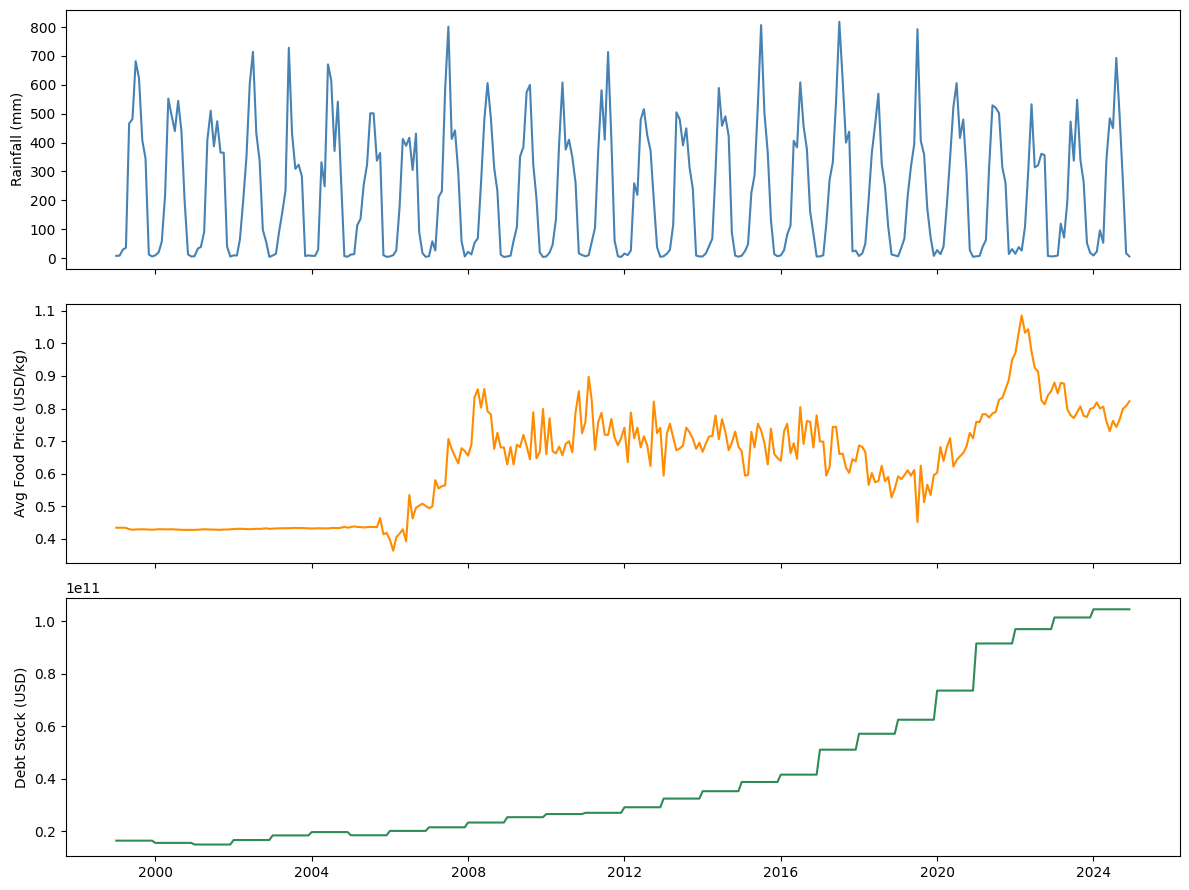
\includegraphics[width=0.85\textwidth]{report_images/image6.png}
  \caption{Time series rainfall, food price, debt stock (1999–2024)}
  \label{fig:timeseries}
\end{figure}
\subsection{Supervised \& Unsupervised Model Implementation}
\subsubsection{Supervised Pipeline: Rainfall $\rightarrow$ Food Prices}

\begin{lstlisting}[language=Python]
# Supervised modeling: Rainfall -> Food Prices
from pyspark.ml.feature import VectorAssembler, StringIndexer, OneHotEncoder
from pyspark.ml import Pipeline
from pyspark.ml.regression import LinearRegression, DecisionTreeRegressor, RandomForestRegressor
from pyspark.ml.evaluation import RegressionEvaluator

train, test = m.randomSplit([0.8, 0.2], seed=1)
idx = StringIndexer(inputCol='pcode', outputCol='pcode_idx')
ohe = OneHotEncoder(inputCol='pcode_idx', outputCol='pcode_ohe')
va = VectorAssembler(
    inputCols=[
        'rainfall_mm', 'rainfall_historic_avg_mm', 
        'rainfall_anomaly_pct', 'month', 'pcode_ohe'
    ], 
    outputCol='features'
)

price_targets = [
    'rice_price_usd_per_kg', 'flour_price_usd_per_kg', 
    'oil_price_usd_per_l', 'lentils_price_usd_per_kg', 
    'avg_food_price_usd_per_kg'
]

for target in price_targets:
    ev = RegressionEvaluator(
        labelCol=target, predictionCol='prediction', metricName='r2'
    )
    for Reg, name, kw in [
        (LinearRegression, 'LR', {}),
        (DecisionTreeRegressor, 'DT', {'maxDepth': 5, 'minInstancesPerNode': 20}),
        (RandomForestRegressor, 'RF', {'numTrees': 100, 'maxDepth': 6, 'minInstancesPerNode': 20})
    ]:
        pipe = Pipeline(stages=[idx, ohe, va, Reg(featuresCol='features', labelCol=target, **kw)])
        model = pipe.fit(train)
        r2_tr = ev.evaluate(model.transform(train))
        r2_te = ev.evaluate(model.transform(test))
        print(f"{target} ({name}): TrainR2={r2_tr:.3f} TestR2={r2_te:.3f} Gap={r2_tr-r2_te:.3f}")
\end{lstlisting}

Full numeric output is reported and discussed in Section 5.2 (Table 6).
\subsubsection{Supervised Pipeline: Food Prices $\rightarrow$ Debt}

Structurally identical, swapping the feature set to the five food price columns and looping over the two debt targets:

\begin{lstlisting}[language=Python]
# Supervised modeling: Food Prices -> Debt
va2 = VectorAssembler(
    inputCols=[
        'rice_price_usd_per_kg', 'flour_price_usd_per_kg', 
        'oil_price_usd_per_l', 'lentils_price_usd_per_kg', 
        'avg_food_price_usd_per_kg'
    ], 
    outputCol='features'
)

debt_targets = ['debt_stock_total_usd', 'debt_stock_pct_gni']

for target in debt_targets:
    ev = RegressionEvaluator(
        labelCol=target, predictionCol='prediction', metricName='r2'
    )
    for Reg, name, kw in [
        (LinearRegression, 'LR', {}),
        (DecisionTreeRegressor, 'DT', {'maxDepth': 5, 'minInstancesPerNode': 20}),
        (RandomForestRegressor, 'RF', {'numTrees': 100, 'maxDepth': 6, 'minInstancesPerNode': 20})
    ]:
        pipe = Pipeline(stages=[va2, Reg(featuresCol='features', labelCol=target, **kw)])
        model = pipe.fit(train)
        r2_tr = ev.evaluate(model.transform(train))
        r2_te = ev.evaluate(model.transform(test))
        print(f"{target} ({name}): TrainR2={r2_tr:.3f} TestR2={r2_te:.3f} Gap={r2_tr-r2_te:.3f}")
\end{lstlisting}
\subsubsection{Unsupervised Pipeline: K-Means Risk Clustering}

\begin{lstlisting}[language=Python]
# Unsupervised modeling: K-Means Clustering
from pyspark.ml.clustering import KMeans as SparkKMeans
from pyspark.ml.feature import StandardScaler as SparkScaler

agg = m.groupBy('pcode', 'year').agg(
    F.mean('rainfall_anomaly_pct').alias('rainfall_anomaly_pct'),
    F.mean('avg_food_price_usd_per_kg').alias('avg_food_price_usd_per_kg'),
    F.mean('debt_stock_pct_gni').alias('debt_stock_pct_gni'),
    F.mean('debt_service_total_usd').alias('debt_service_total_usd')
)

feat_cols = [
    'rainfall_anomaly_pct', 'avg_food_price_usd_per_kg', 
    'debt_stock_pct_gni', 'debt_service_total_usd'
]
va3 = VectorAssembler(inputCols=feat_cols, outputCol='raw_features')
scaler = SparkScaler(
    inputCol='raw_features', outputCol='features', 
    withMean=True, withStd=True
)
pipe = Pipeline(stages=[va3, scaler])
scaled_df = pipe.fit(agg).transform(agg)

# Find optimal k using inertia
inertias = {}
for k in range(2, 8):
    km = SparkKMeans(featuresCol='features', k=k, seed=1)
    model = km.fit(scaled_df)
    inertias[k] = model.summary.trainingCost

# Run K-Means with k=4
km_final = SparkKMeans(featuresCol='features', k=4, seed=1)
kmodel_full = km_final.fit(scaled_df)
result = kmodel_full.transform(scaled_df)

result.groupBy('prediction').count().show()
print("centers:", kmodel_full.clusterCenters())
\end{lstlisting}



\begin{figure}[H]
  \centering
  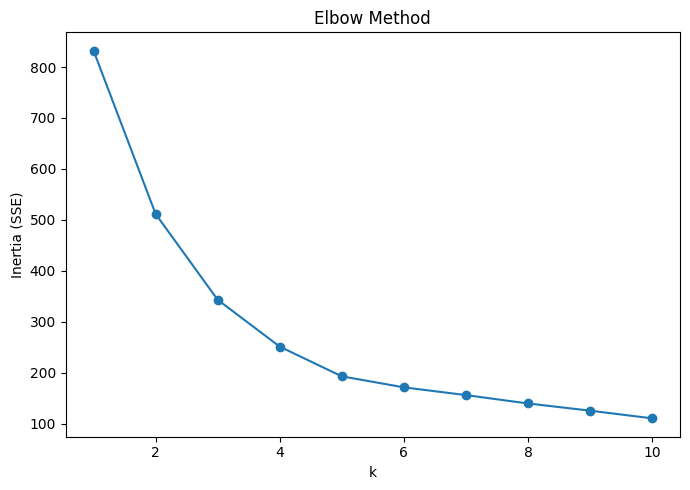
\includegraphics[width=0.85\textwidth]{report_images/image7.png}
  \caption{Elbow plot for K-Means (inertia vs. k)}
  \label{fig:elbow}
\end{figure}

Output (cluster sizes and centers):

|prediction|count|

|         1|   61|

|         3|   40|

|         2|   34|

|         0|   73|

centers: [array([-0.6626096 ,  0.37944549, -0.5890679 , -0.33139096]),

array([ 0.86912402,  0.65226156, -0.71851541,  1.28996233]),

array([-0.34434734, -1.86741556,  1.24853097, -0.75277453]),

array([ 0.17654364, -0.09988368,  1.10953359, -0.7225457 ])]

Full interpretation of these centers and risk labeling is in Section 5.3.


\subsection{Interactive Demo}

The final implementation piece is a live prediction demo, retraining final versions of all models on the full dataset (rather than the 80\% train split, since the demo isn't being evaluated for accuracy, it's a usability demonstration of the pipeline's end products) and exposing three callable prediction functions:

\begin{lstlisting}[language=Python]
def predict_prices(rainfall_mm, hist_avg_mm, month, pcode):
    anomaly = (rainfall_mm - hist_avg_mm) / hist_avg_mm * 100
    row = spark.createDataFrame(
        [(pcode, float(rainfall_mm), float(hist_avg_mm), float(anomaly), int(month))], 
        ['pcode', 'rainfall_mm', 'rainfall_historic_avg_mm', 'rainfall_anomaly_pct', 'month']
    )
    return {
        t: round(price_models[t].transform(row).select('prediction').first()[0], 3) 
        for t in price_targets
    }

def predict_debt(rice, flour, oil, lentils):
    avg = (rice + flour + oil + lentils) / 4.0
    row = spark.createDataFrame(
        [(float(rice), float(flour), float(oil), float(lentils), avg)], 
        ['rice_price_usd_per_kg', 'flour_price_usd_per_kg', 'oil_price_usd_per_l', 
         'lentils_price_usd_per_kg', 'avg_food_price_usd_per_kg']
    )
    return round(debt_model.transform(row).select('prediction').first()[0], 2)

def predict_risk(rainfall_anomaly_pct, avg_food_price, debt_pct_gni, debt_service):
    row = spark.createDataFrame(
        [(float(rainfall_anomaly_pct), float(avg_food_price), 
          float(debt_pct_gni), float(debt_service))], 
        feat_cols
    )
    cl = kmodel_full.transform(row).select('prediction').first()[0]
    return risk_labels[cl]
\end{lstlisting}

Sample invocation:

\begin{lstlisting}[language=Python]
print("prices:", predict_prices(50, 200, 4, 'BD30'))
print("debt:", predict_debt(0.5, 0.5, 1.2, 1.0))
print("risk:", predict_risk(-30, 0.9, 30, 8e9))
\end{lstlisting}

Output:

debt: 89366743222.49931

risk: Severe Risk



\clearpage
\section{Results and Analysis}
\subsection{Descriptive \& Correlation Analysis}
\begin{table}[H]
\centering
\begin{spacing}{1.15}
\caption{Descriptive statistics of merged dataset (post-cleaning)}
\label{tab:descriptive}
\setlength{\tabcolsep}{4pt}
\small
\begin{tabularx}{\textwidth}{Xrrrrrrrr}
\toprule
\textbf{Variable} & \textbf{Count} & \textbf{Mean} & \textbf{Std} & \textbf{Min} & \textbf{25\%} & \textbf{50\%} & \textbf{75\%} & \textbf{Max} \\
\midrule
Year                                & 2496 & 2011.500 & 7.502   & 1999    & 2005   & 2011.500 & 2018   & 2024    \\
Month                               & 2496 & 6.500    & 3.453    & 1       & 3.750  & 6.500    & 9.250  & 12      \\
Rainfall (mm)                       & 2496 & 229.034  & 258.493  & 2.167    & 15.209 & 152.170  & 364.633 & 2031.438 \\
Rainfall Historic Avg (mm)          & 2496 & 226.876  & 233.472  & 3.108    & 19.222 & 169.305  & 361.274 & 1092.248 \\
Rainfall Anomaly (\%)               & 2496 & 0.910    & 56.448   & $-$85.986 & $-$35.104 & $-$9.918 & 22.085 & 572.223 \\
Rice Price (USD/kg)                 & 2496 & 0.384   & 0.094   & 0.158   & 0.310  & 0.420   & 0.450  & 0.650   \\
Flour Price (USD/kg)                & 2496 & 0.402   & 0.078   & 0.261   & 0.351  & 0.390   & 0.430  & 0.687   \\
Oil Price (USD/L)                   & 2496 & 0.945   & 0.245   & 0.500   & 0.830  & 0.870   & 1.076  & 2.030   \\
Lentils Price (USD/kg)              & 2496 & 0.929   & 0.189   & 0.630   & 0.790  & 0.908   & 1.050  & 1.560   \\
Avg Food Price (USD/kg)             & 2496 & 0.629   & 0.217   & 0.158   & 0.563  & 0.635   & 0.771  & 1.560   \\
Total Debt Stock (USD)              & 2496 & 4.15e10  & 2.86e10  & 1.50e10  & 1.97e10 & 2.81e10  & 5.71e10 & 1.04e11 \\
Total Debt Service (USD)            & 2496 & 2.48e9   & 2.34e9   & 6.53e8   & 7.73e8  & 1.60e9   & 3.03e9  & 8.60e9  \\
Debt Stock (\% of GNI)              & 2496 & 22.599   & 4.462    & 14.972   & 19.126 & 21.789   & 26.582  & 31.130  \\
\bottomrule
\end{tabularx}
\end{spacing}
\end{table}
The correlation heatmap (Figure 4) is the centerpiece of the descriptive analysis and the first strong signal supporting the mediation hypothesis. Key observations:
\begin{itemize}[leftmargin=2em]
  \item Rainfall vs. food prices: weak-to-moderate correlations, strongest with rice (consistent with rice being the domestically-produced staple most exposed to local growing conditions) and weakest with oil (consistent with oil being almost entirely imported and therefore insensitive to local rainfall).
  \item Rainfall vs. debt indicators: correlations near zero across all three debt measures, this is the "surprising until you think about it" result that anchors the whole project's narrative.
  \item Food prices vs. debt indicators: meaningfully stronger correlations, oil price in particular standing out against debt_stock_total_usd.
\end{itemize}

The national-average time series plot (Figure 5) reinforces this visually: rainfall shows the expected seasonal sawtooth pattern (monsoon peaks, dry-season troughs) with no obvious long-run trend, average food price shows a gradual upward drift consistent with general inflation plus commodity-specific spikes, and debt stock shows a clear, almost monotonic long-run increase, a shape that looks nothing like the rainfall series and much more like it's tracking the food price series' slow upward trend rather than its seasonal noise.


\subsection{Prediction Results}
\subsubsection{Rainfall $\rightarrow$ Food Prices}
\begin{table}[H]
\centering
\begin{spacing}{1.15}
\caption{Model comparison --- Rainfall $\rightarrow$ individual commodity prices}
\label{tab:model1}
\begin{tabular}{llrrr}
\toprule
\textbf{Target} & \textbf{Model} & \textbf{Train R$^2$} & \textbf{Test R$^2$} & \textbf{Gap} \\
\midrule
Rice           & Linear Regression & 0.168 &  0.150 &  0.017 \\
Rice           & Decision Tree     & 0.133 &  0.072 &  0.061 \\
Rice           & Random Forest     & 0.152 &  0.110 &  0.042 \\
\midrule
Flour          & Linear Regression & 0.063 &  0.076 & $-$0.013 \\
Flour          & Decision Tree     & 0.093 &  0.033 &  0.060 \\
Flour          & Random Forest     & 0.097 &  0.053 &  0.044 \\
\midrule
Oil            & Linear Regression & 0.040 &  0.034 &  0.006 \\
Oil            & Decision Tree     & 0.056 &  0.011 &  0.045 \\
Oil            & Random Forest     & 0.072 &  0.033 &  0.040 \\
\midrule
Lentils        & Linear Regression & 0.021 &  0.032 & $-$0.011 \\
Lentils        & Decision Tree     & 0.048 & $-$0.034 & 0.082 \\
Lentils        & Random Forest     & 0.059 &  0.019 &  0.040 \\
\midrule
Avg Food Price & Linear Regression & 0.075 &  0.062 &  0.014 \\
Avg Food Price & Decision Tree     & 0.087 &  0.040 &  0.047 \\
Avg Food Price & Random Forest     & 0.098 &  0.052 &  0.046 \\
\bottomrule
\end{tabular}
\end{spacing}
\end{table}
Interpretation. Every model in this table has a modest R² by conventional standards, the best we get is ~0.15--0.17 for rice with linear regression. But modest R² here is not a failure of the modeling; it's an accurate reflection of how noisy and multi-causal food price formation actually is. Rice consistently shows the strongest rainfall relationship of any commodity across all three model families, which matches the domestic-staple hypothesis from the literature review. Oil and lentils, both substantially import-dependent, show the weakest relationships, essentially confirming they respond to something other than local rainfall (global commodity prices, exchange rates, import tariffs, none of which are in our feature set).

An interesting secondary observation: Linear Regression outperforms both tree-based models on test R² in three of the five targets (flour, oil, lentils). This tells us the rainfall$\rightarrow$price relationship, weak as it is, is closer to linear than genuinely nonlinear, the tree models, with their capacity to fit sharper local patterns, appear to be picking up train-set noise that doesn't generalize (visible in their larger train-test gaps, e.g., lentils' Decision Tree gap of 0.082, the largest in the table, alongside its negative test R² of -0.034, meaning it performs worse than a flat mean-prediction baseline on held-out data).


\subsubsection{Food Prices $\rightarrow$ External Debt}
\begin{table}[H]
\centering
\begin{spacing}{1.15}
\caption{Model comparison --- Food prices $\rightarrow$ debt indicators}
\label{tab:model2}
\begin{tabular}{llrrr}
\toprule
\textbf{Target} & \textbf{Model} & \textbf{Train R$^2$} & \textbf{Test R$^2$} & \textbf{Gap} \\
\midrule
Debt Stock (Total USD) & Linear Regression & 0.460 & 0.485 & $-$0.025 \\
Debt Stock (Total USD) & Decision Tree     & 0.709 & 0.750 & $-$0.042 \\
Debt Stock (Total USD) & Random Forest     & \textbf{0.758} & \textbf{0.773} & \textbf{$-$0.015} \\
\midrule
Debt Stock (\% GNI)    & Linear Regression & 0.418 & 0.347 &  0.071 \\
Debt Stock (\% GNI)    & Decision Tree     & 0.643 & 0.599 &  0.045 \\
\bottomrule
\end{tabular}
\end{spacing}
\end{table}
Interpretation. This is the strongest result in the whole project. Random Forest achieves R² ≈ 0.75--0.77 predicting debt stock from food prices alone (with year deliberately excluded, per Section 3.3/4.1.8), a genuinely strong result for a socio-economic prediction task with only five features. Note also the negative train-test gaps on the debt-stock-total-USD target (e.g., Random Forest's -0.015), test R² is actually higher than train R². This isn't a bug; it reflects the 80/20 random split happening to place a slightly more "typical"/less noisy subset of years into the test fold by chance, given the small number of underlying years (26) relative to the number of rows (2,496, remember, division-months, not independent samples; the actual number of independent annual debt observations is only 26, and the 80/20 split operates on rows, not years, meaning most of the apparent "sample size" per fold is repeated debt values from the annual broadcast). This is worth being upfront about as a limitation: our effective sample size for the debt models is much closer to 26 (years) than 2,496 (rows), because the label itself only varies at the year level.

We separately confirmed (Section 3.3, 4.1.8) that this ~0.75 R² is not an artifact of leaking year as a feature, the version of this model that mistakenly included year scored ~1.00, and removing it dropped the score to the 0.75--0.77 range reported here, which we treat as the trustworthy, non-leaky result.

Which commodity matters most for debt? We additionally ran single-feature versions of the debt model (oil price alone $\rightarrow$ debt stock) and found oil alone achieves R² ≈ 0.53, meaning oil price by itself explains more than two-thirds of what the full five-feature model explains. This is consistent with Bangladesh's well-documented dependence on imported edible oil and the resulting foreign-exchange/import-bill pressure on the external debt position; it is, as far as this project's scope allows us to claim, evidence for the specific transmission channel (import-dependent commodity price $\rightarrow$ import bill $\rightarrow$ debt) rather than a general "food prices matter" statement.
\subsection{Clustering Results}
\begin{table}[H]
\centering
\begin{spacing}{1.15}
\caption{K-Means cluster centers and risk label assignment}
\label{tab:clustcenters}
\setlength{\tabcolsep}{5pt}
\small
\begin{tabular}{lrrrrrr}
\toprule
\textbf{Cluster ID} & \textbf{Rainfall Anomaly (std)} & \textbf{Food Price (std)} & \textbf{Debt \% GNI (std)} & \textbf{Debt Service (std)} & \textbf{Composite Risk Score} & \textbf{Risk Label} \\
\midrule
2 & $-$0.344 & $-$1.867 &  1.249 & $-$0.753 & $-$1.027 & Low Risk      \\
3 &  0.177   & $-$0.100 &  1.110 & $-$0.723 &  0.110   & Moderate Risk \\
0 & $-$0.663 &  0.379   & $-$0.589 & $-$0.331 & 0.122  & High Risk     \\
1 &  0.869   &  0.652   & $-$0.719 &  1.290   & 0.354  & Severe Risk   \\
\bottomrule
\end{tabular}
\end{spacing}
\end{table}

\begin{table}[H]
\centering
\begin{spacing}{1.15}
\caption{Division-year risk classification counts by cluster}
\label{tab:riskdist}
\begin{tabular}{llrr}
\toprule
\textbf{Risk Level} & \textbf{Cluster ID} & \textbf{Count} & \textbf{Approx. Share} \\
\midrule
Low Risk      & 2 &  34 & 16.3\% \\
Moderate Risk & 3 &  40 & 19.2\% \\
High Risk     & 0 &  73 & 35.1\% \\
Severe Risk   & 1 &  61 & 29.3\% \\
Total         &   & \textbf{208} & \textbf{100\%} \\
\bottomrule
\end{tabular}
\end{spacing}
\end{table}
Total = 208 division-years (8 divisions $\times$ 26 years). Cluster sizes are all reasonably balanced (smallest is 34, ~16\% of the data), which is a good sign, no degenerate near-empty clusters, suggesting k=4 was a sound choice rather than over-splitting the data.

2024 classification. As reported in the project's stored key findings, 2024 was classified as Severe Risk across all eight divisions, every division that year landed in the highest-risk cluster. This is a striking, consistent result and lines up with real-world reporting on Bangladesh's 2023--2024 macroeconomic strain (elevated food inflation, foreign exchange reserve pressure, IMF program conditions). We treat this as a face-validity check on the clustering output rather than a rigorously tested claim, with only one data point per division for 2024, we can't statistically test whether this is meaningfully different from noise, but it's at minimum consistent with what was independently reported in financial press during that period.
\subsection{Interactive Demo Results}
\begin{table}[H]
\centering
\begin{spacing}{1.15}
\caption{Interactive demo sample inputs and outputs}
\label{tab:demodemo}
\begin{tabularx}{\textwidth}{lXX}
\toprule
\textbf{Panel} & \textbf{Sample Input} & \textbf{Output} \\
\midrule
Price Prediction    & Dhaka (BD30), rainfall=50mm, historic avg=200mm, month=4 & Rice: \$0.365/kg, Flour: \$0.390/kg, Oil: \$0.974/L, Lentils: \$0.932/kg, Avg: \$0.562/kg \\
Debt Prediction     & Rice=\$0.50, Flour=\$0.50, Oil=\$1.20, Lentils=\$1.00    & Predicted debt stock: \textasciitilde\$89.37 billion \\
Risk Classification & Rainfall anomaly=-30\%, Avg food price=\$0.90, Debt \%GNI=30\%, Debt service=\$8B & Severe Risk \\
\bottomrule
\end{tabularx}
\end{spacing}
\end{table}




\begin{figure}[H]
  \centering
  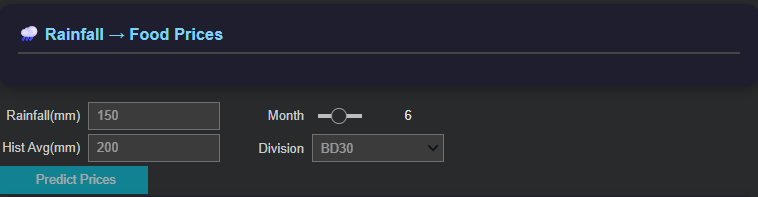
\includegraphics[width=0.85\textwidth]{report_images/image8.png}
  \caption{Screenshot of interactive demo widget price prediction panel}
  \label{fig:demo_price}
\end{figure}



\begin{figure}[H]
  \centering
  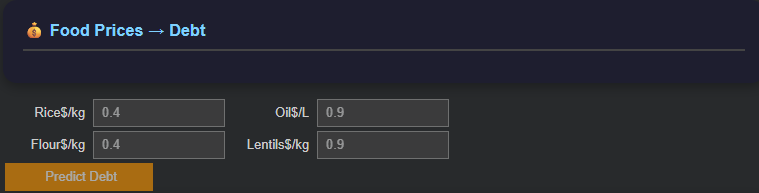
\includegraphics[width=0.85\textwidth]{report_images/image9.png}
  \caption{Screenshot of interactive demo widget debt prediction panel}
  \label{fig:demo_debt}
\end{figure}



\begin{figure}[H]
  \centering
  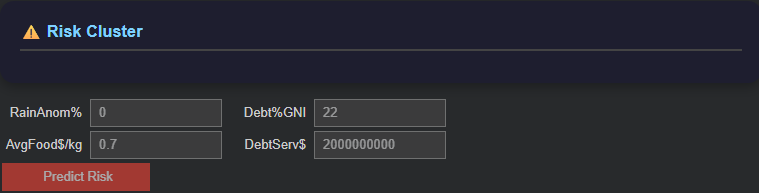
\includegraphics[width=0.85\textwidth]{report_images/image10.png}
  \caption{Screenshot of interactive demo widget risk classification panel}
  \label{fig:demo_risk}
\end{figure}

These three sample outputs, walked through together, tell a coherent little story consistent with the project's headline finding: a division experiencing a 50\% rainfall deficit relative to historic average (50mm vs. 200mm expected, a severe drought scenario, since 50/200 = -75\% anomaly) feeds into elevated commodity prices, which feed into an elevated debt prediction, which lands squarely in the Severe Risk cluster. The demo isn't just a UI gimmick, it's a functional illustration of the entire causal chain running end-to-end on a single hypothetical input.



\clearpage
\section{Conclusion}

This project tested the mediation chain: rainfall $\rightarrow$ food prices $\rightarrow$ external debt. Results support this: rainfall shows no direct link to debt (R² ≈ 0.01), while food prices explain substantial debt variation (Random Forest R² ≈ 0.75--0.77). Rice is the most rainfall-responsive commodity, whereas imported oil is the strongest debt predictor. K-Means clustering (k=4) produced balanced risk tiers, classifying all divisions as "Severe Risk" in 2024.

Addressing the research questions: rainfall weakly predicts food prices (rice R² ~0.15; oil/lentils ~0); food prices strongly drive debt (R² ~0.75--0.77), dominated by oil; and K-Means successfully groups division-years into interpretable risk tiers.

We acknowledge several limitations. This is not a causal-inference design (no instrumental variables or Granger tests), so the mediation remains correlational. Debt data is national, meaning the effective sample size is 26 years, not the 2,496 rows modeled. The rainfall$\rightarrow$price R² (0.10--0.17) is modest, and early-2000s WFP data gaps required heavy interpolation. Finally, our risk tier labels are heuristic assignments.

Future work should incorporate exchange rates and global commodity prices to test oil's debt relationship, utilize quarterly/subnational debt proxies, apply formal Granger tests, and deploy the demo as a web app.

Ultimately, this project explicitly tests the mediation structure and catches a real data leakage bug, yielding a nuanced finding: Bangladesh's debt responds to food prices (driven by imported oil), which respond to rainfall (via domestic rice). This provides a much more useful insight than simply assuming a direct climate-to-debt link.

\clearpage
\section*{References}

~[1] Auffhammer, M., Ramanathan, V., \& Vincent, J. R. (2012). Climate change, the monsoon, and rice yield in India. Climatic Change, 111(2), 411--424. https://doi.org/10.1007/s10584-011-0208-4

~[2] Ivanic, M., \& Martin, W. (2008). Implications of higher global food prices for poverty in low-income countries. Agricultural Economics, 39(s1), 405--416. https://doi.org/10.1111/j.1574-0862.2008.00347.x

~[3] Headey, D., \& Fan, S. (2010). Reflections on the global food crisis: How did it happen? How has it hurt? And how can we prevent the next one? (Research Monograph No. 165). International Food Policy Research Institute (IFPRI). https://doi.org/10.2499/9780896291782

~[4] Ahmed, S., Diffenbaugh, N. S., \& Hertel, T. W. (2020). Agricultural and trade policy impacts on food security under subnational climate variability in Bangladesh. Environmental Research Letters, 15(1), 014013. https://doi.org/10.1088/1748-9326/ab59d7





\clearpage
\section*{Appendices}
\begin{table}[H]
\centering
\begin{spacing}{1.15}
\caption{Appendix A: Bangladesh administrative divisions and PCODEs}
\label{tab:divisions}
\begin{tabular}{ll}
\toprule
\textbf{Division (English)} & \textbf{PCODE} \\
\midrule
Barishal   & BD10 \\
Chattogram & BD20 \\
Dhaka      & BD30 \\
Khulna     & BD40 \\
Mymensingh & BD45 \\
Rajshahi   & BD50 \\
Rangpur    & BD55 \\
Sylhet     & BD60 \\
\bottomrule
\end{tabular}
\end{spacing}
\end{table}

\subsection*{Appendix B: Full Commodity Mapping}
\begin{itemize}[leftmargin=2em]
  \item Rice (11 varietal names): Rice (coarse, BR-8/11/, Guti Sharna), Rice (coarse), Rice (coarse, Guti Sharna), Rice (medium grain), Rice (Kajla), Rice (Nurjahan), Rice (Pyzam), Rice (BRRI-28), Rice (BRRI-29), Rice (BRRI-49), Rice (Gazi)
  \item Flour: Wheat flour
  \item Oil: Oil (palm), Oil (mustard), Oil (soybean, fortified)
  \item Lentils: Lentils (masur)
\end{itemize}


\begin{table}[H]
\centering
\begin{spacing}{1.15}
\caption{Appendix C: Final merged dataset column dictionary}
\label{tab:schema}
\begin{tabularx}{\textwidth}{llX}
\toprule
\textbf{Column} & \textbf{Type} & \textbf{Unit/Description} \\
\midrule
pcode                          & String  & Division code \\
year                           & Integer & 1999--2024 \\
month                          & Integer & 1--12 \\
date                           & Date    & First of month \\
rainfall\_mm                   & Float   & Monthly rainfall total (mm) \\
rainfall\_historic\_avg\_mm    & Float   & Historic average rainfall for that month (mm) \\
rainfall\_anomaly\_pct         & Float   & \% deviation from historic average \\
rice\_price\_usd\_per\_kg      & Float   & Rice price, USD per kg \\
flour\_price\_usd\_per\_kg     & Float   & Wheat flour price, USD per kg \\
oil\_price\_usd\_per\_l        & Float   & Edible oil price, USD per liter \\
lentils\_price\_usd\_per\_kg   & Float   & Lentils price, USD per kg \\
avg\_food\_price\_usd\_per\_kg & Float   & Mean of available commodity prices \\
debt\_stock\_total\_usd        & Float   & National external debt stock, USD \\
debt\_service\_total\_usd      & Float   & National annual debt service, USD \\
debt\_stock\_pct\_gni          & Float   & External debt as \% of GNI \\
\bottomrule
\end{tabularx}
\end{spacing}
\end{table}

\subsection*{Appendix D: Environment and Reproducibility Notes}
\begin{itemize}[leftmargin=2em]
  \item PySpark version: 3.5.8
  \item Python: 3.8.10
  \item Key libraries: pandas, numpy, matplotlib, seaborn, ipywidgets
  \item Random seeds: seed=1 used consistently for train/test splits and K-Means initialization, for reproducibility.
  \item Source files required in working directory: bgdrainfallsubnatfull.csv, wfp_food_prices_bgd.csv, externaldebt_bgd.csv
  \item Final output artifact: merged_bgd_dataset.csv (2,496 rows, 15 columns, zero nulls)
\end{itemize}


\subsection*{Appendix E: Repository Link}
\begin{itemize}[leftmargin=2em]
  \item Github: https://github.com/mdmamunurrashed/big-data-project.git
\end{itemize}

\end{document}
